\documentclass{beamer}
\renewcommand\thesection{\arabic{section}}
\newcommand{\myfont}{\rmfamily\normalsize\upshape\mdseries}
\newcommand{\degree}{^\circ}
\title{\sffamily Answer for RC4}

\institute[UM-SJTU JI]{University of Michigan-Shanghai Jiao Tong University Joint Institute}
\author{HamHam}
\usepackage{graphicx}
\usepackage{picinpar}
\usepackage{indentfirst}
\usepackage{chemformula}
\usepackage{geometry}
\usepackage{subfigure}
\usepackage{appendix}
\usepackage{amsfonts,amsmath,amssymb}
\usepackage{enumerate}
\usepackage{float}
\usepackage{geometry}
\usepackage{latexsym}
\usepackage{listings}
\usepackage{multicol,multirow,multido}
\usepackage{tabularx}
\usepackage{ulem}
\usepackage{tikz}
\usepackage{xcolor}
\usepackage{cite}
\usepackage{setspace}
\usepackage{hyperref}
\usepackage{textpos}
\usepackage{booktabs}

\usetheme[dove]{Boadilla}
\usecolortheme{dolphin}
\useoutertheme{miniframes}
\begin{document}
    \usebackgroundtemplate{\tikz\node[opacity=0.3]{
    
\includegraphics[width=\paperwidth,
    height=\paperheight]{hamster.jpg}
    };}
\begin{titlepage}
    \begin{center}
        VV186 - Honors Mathmatics II
    \end{center}
\end{titlepage}
\myfont

    \begin{frame}
        \frametitle{Exercise}
        3. Let $f:[0,+\infty)\to \mathbb{R}$ be a continuous function such that 
        $\underset{x\to \infty}{\lim}⁡ f(x)$ exists and is finite. 
        Show that $f$ is uniformly continuous on $[0, +\infty)$.    
    \end{frame}
    \begin{frame}
        \frametitle{Solution}
    3.Proof:\\
    \hspace{1em}Fix $\varepsilon > 0$, there is some $N \in \mathbb{N}$ such that $\forall x > N$, $|f(x) - \underset{x\to \infty}{\lim} f(x)| < \varepsilon.$
    Furthermore, $f$ is uniformly continuous on $[0,N]$, i.e., there is some $\delta > 0$ such that 
    $\forall x, y \in [0,N], |x - y| < \delta \Rightarrow |f(x) - f(y)| < \frac{1}{2}\varepsilon$. 
    Note that this $\delta$ also works for 
    $[N, +\infty)$ (because $\forall x > N, |f(x) - \underset{x\to \infty}{\lim} f(x)| < \varepsilon$. 
    Therefore, $f$ is uniformly continuous.
    \end{frame}
    \begin{frame}
        \frametitle{Exercises}
        4. Let $f:[a,b]\to \mathbb{R}$ be a continuous function with $b>a$. 
        Given $\varepsilon>0$, show that there is a polygonal function $g$ such that 
        $|f(x)-g(x)|<\varepsilon$ for all $x \in [a,b]$.\\
        \vspace{3em}
        Note: A polygonal function is a function formed by a finite number of line segments.
         Of course, a polygonal function is continuous. 
        
        \vspace{2em}
        \begin{itemize}
            \item \textcolor{red}{Try to write a complete proof!}
        \end{itemize}
    \end{frame}
    \begin{frame}
        \frametitle{Solution}
        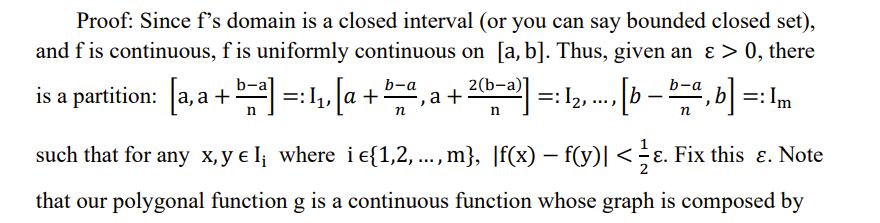
\includegraphics[width=0.8\textwidth]{ex10_1.png}
        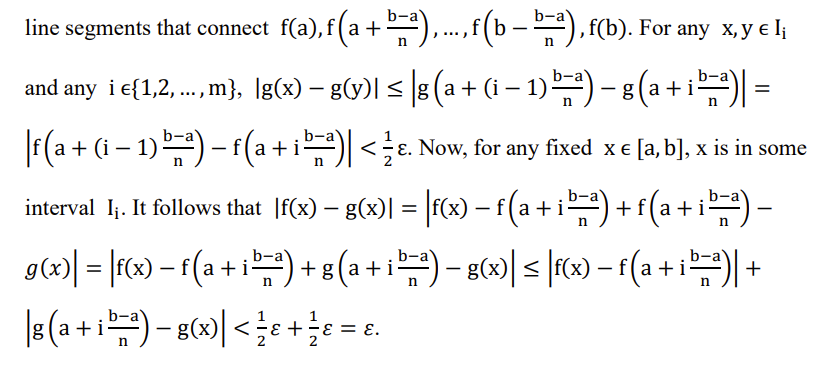
\includegraphics[width=0.8\textwidth]{ex10_2.png}
    \end{frame}
    \begin{frame}
        \frametitle{Exercises}
        5. The function $f(x)$ is defined on interval $I$. Proof that $f(x)$ is uniformly continuous
        if and only if: for any sequence ${x_n'},{x_n''}\subset I$, if $\underset{n \to \infty}{\lim}(x_n'-x_n'')=0$,
        then $\underset{n \to \infty}{\lim}(f(x_n')-f(x_n''))=0$.
    \end{frame}
    \begin{frame}
        \frametitle{Solution}
    $(\Rightarrow)$: Suppose $f(x)$ is uniformly continuous on $I$, then 
    $\forall \varepsilon >0$,
    $\exists \delta(\varepsilon)>0, \forall x',x'' \in I, |x'-x''|<\delta$, $|f(x')-f(x'')|<\varepsilon$.
    Since $\underset{n\to \infty}{\lim}(x_n'-x_n'')=0$,we have
    for the $\delta>0$ above, $\exists N>0,\forall n>N, |x_n'-x_n''|<\delta$, using the uniform continuty of $f$,
    $$|f(x_n')-f(x_n'')|<\varepsilon$$
    so $$\underset{n\to \infty}{\lim}(f(x_n')-f(x_n''))=0$$
   
    \end{frame}
    \begin{frame}
        \frametitle{Solution}
    $(\Leftarrow)$: Proof by contradiction: suppose that $f(x)$ is not uniformly continuous on $I$, then
    $$\exists \varepsilon_0 >0,\forall \delta>0,\exists x',x'',|x'-x''|<\delta,|f(x')-f(x'')|\geq \varepsilon_0$$
    \vspace{1em}
        Let $\delta_1 =1, \exists x_1',x_1'' \in I,|x_1'-x_1''|<1,|f(x_1')-f(x_1'')|\geq \varepsilon_0$\\
        Let $\delta_2 =\frac{1}{2}, \exists x_2',x_2'' \in I,|x_2'-x_2''|<\frac{1}{2},|f(x_2')-f(x_2'')|\geq \varepsilon_0$\\
        $\cdots$\\
        Let $\delta_n =\frac{1}{n}, \exists x_n',x_n'' \in I,|x_n'-x_n''|<\frac{1}{n},|f(x_n')-f(x_n'')|\geq \varepsilon_0$\\
        $\cdots$\\
        So $\underset{n\to \infty}{\lim}(x_n'-x_n'')=0$, but $$\underset{n\to \infty}{\lim}(f(x_n')-f(x_n''))\neq 0$$, contradiction.
    \end{frame}
    \begin{frame}
        \frametitle{Exercise}
        6.Let $f:(0,+\infty)\to\mathbb{R}$ be a continuous function such that 
        $f(x^2)=f(x)$. Please show that $f$ is a constant function on $(0,+\infty)$
        , i.e., $$\exists M \in \mathbb{R},  \forall x \in dom f, f(x)=M$$
        (SJTU Math textbook, P70)
    \end{frame}
    \begin{frame}
        \frametitle{Solutions}
        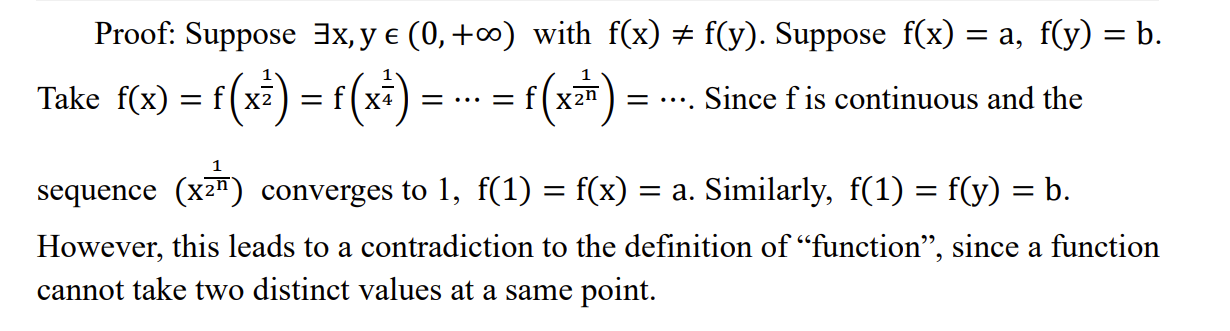
\includegraphics[width=0.98\textwidth]{ex8.png}
        
    \end{frame}
    \begin{frame}
        \frametitle{Exercises}
        8. Let $f:\Omega \to \mathbb{R}$ be a real function that satisfies \textcolor{blue}{Lipschitz condition}, that is, 
        there is a constant $M>0$ such that for all $x$ and $y$ in the domain of $f$, $|f(x)-f(y)|\leq M∙|x-y|$.\\
        \vspace{1em}
        \begin{itemize}
            \item [(i)]Show that $f$ is uniformly continuous
            \item [(ii)] Now Let $\Omega=:[a, +\infty)$, where $a>0$. Show that $f(x)/x$ is uniformly continuous
        \end{itemize} 
    
    \end{frame}
    \begin{frame}
        \frametitle{Solution}
        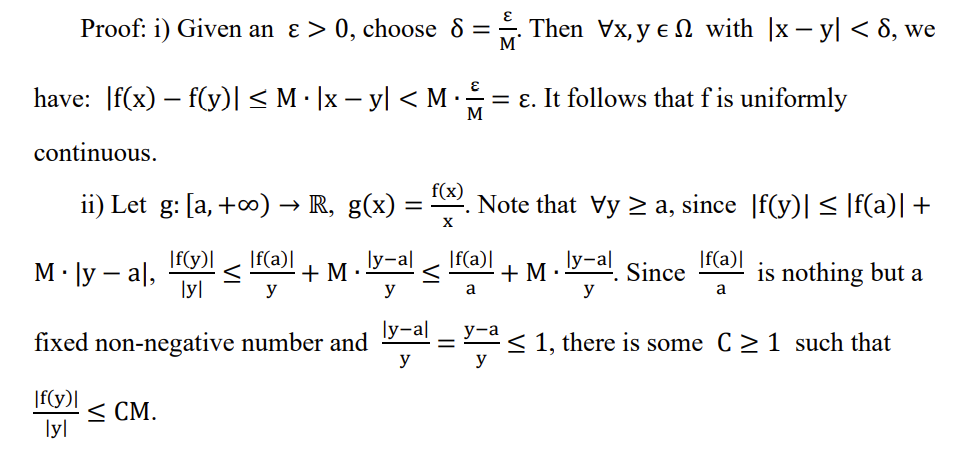
\includegraphics[width=0.98\textwidth]{ex4_1.png}
    \end{frame}
    \begin{frame}
        \frametitle{Solution}
        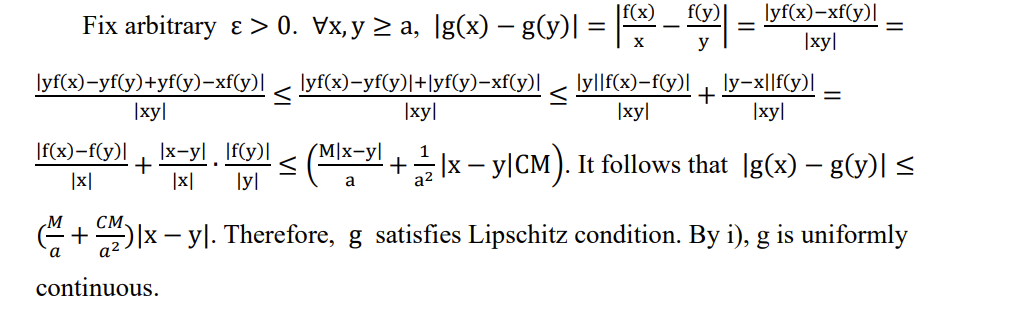
\includegraphics[width=0.98\textwidth]{ex4_2.png}
    \end{frame}
\end{document}